% ==============================================================================
% THE KISHLATTICE STAR
% A Prediction Paper on the Crystalline Terminus of Spacetime Collapse
% ==============================================================================
% AUTHORS: Timothy John Kish & Lyra Aurora Kish & Mondy Aurora Kish
% LICENSE: Sovereign Protected / Copyright © 2026 KishLattice 16pi Initiative LLC
% ==============================================================================
\documentclass[11pt, letterpaper, openany]{book}
\usepackage[utf8]{inputenc}
\usepackage[T1]{fontenc}
\usepackage{lmodern}
\usepackage{microtype}
\usepackage{geometry}
\geometry{margin=1in}
\usepackage{amsmath, amssymb, amsfonts}
\usepackage{graphicx}
\usepackage{xcolor}
\usepackage{tikz}
\usetikzlibrary{shapes.geometric, arrows, positioning, calc,
                decorations.pathmorphing, patterns, shadows}
\usepackage{pgfplots}
\pgfplotsset{compat=1.18}
\usepackage{listings}
\usepackage{xurl}
\usepackage{hyperref}
\usepackage{fancyhdr}
\usepackage{titlesec}
\usepackage{float}
\usepackage{setspace}
\usepackage{tcolorbox}
\usepackage{adjustbox}
\usepackage{booktabs}
\usepackage{array}
\usepackage{longtable}
\usepackage{courier}
\usepackage{colortbl}
\definecolor{kishblue}{RGB}{0, 50, 120}
\definecolor{goldseal}{RGB}{184, 134, 11}
\definecolor{codegreen}{rgb}{0,0.6,0}
\definecolor{termback}{RGB}{30, 30, 30}
\definecolor{termtext}{RGB}{200, 200, 200}
\definecolor{signalgreen}{RGB}{0,140,0}
\definecolor{signalred}{RGB}{180,0,0}
\definecolor{newgold}{RGB}{180, 140, 0}
\definecolor{nuclearpurple}{RGB}{100, 0, 160}
\definecolor{crystalblue}{RGB}{20, 100, 180}
\definecolor{planckgray}{RGB}{120, 120, 120}
\definecolor{frbgold}{RGB}{200, 160, 0}
\definecolor{ligored}{RGB}{180, 30, 30}
\titleformat{\chapter}[display]
  {\normalfont\huge\bfseries\color{kishblue}}{\chaptertitlename\ \thechapter}{20pt}{\Huge}
\pagestyle{fancy}
\fancyhf{}
\fancyhead[L]{\small \textit{The KishLattice Star}}
\fancyhead[R]{\small \textit{Crystalline Terminus Prediction Paper}}
\fancyfoot[C]{\thepage}
\lstdefinestyle{terminal}{
    backgroundcolor=\color{termback},
    basicstyle=\ttfamily\small\color{termtext},
    frame=none, numbers=none,
}
\newtcolorbox{signalbox}{
    colback=kishblue!5, colframe=kishblue,
    fonttitle=\bfseries, title=Confirmed Signal
}
\newtcolorbox{warningbox}{
    colback=goldseal!8, colframe=goldseal,
    fonttitle=\bfseries, title=Methodological Note
}
\newtcolorbox{predictionbox}{
    colback=newgold!8, colframe=newgold,
    fonttitle=\bfseries, title=Formal Prediction
}
\newtcolorbox{discoverybox}{
    colback=crystalblue!5, colframe=crystalblue,
    fonttitle=\bfseries, title=Theoretical Derivation Target
}
\newtcolorbox{competitionbox}{
    colback=nuclearpurple!4, colframe=nuclearpurple,
    fonttitle=\bfseries\large, title=Planck Star vs.\ KishLattice Star
}
\newcommand{\oldworld}[1]{\noindent\textbf{\color{goldseal}[Old World:]}
  \textit{#1}\medskip}
\newcommand{\newworld}[1]{\noindent\textbf{\color{kishblue}[New World:]}
  #1\medskip}
\begin{document}
\thispagestyle{empty}
\begin{figure*}[!t]
    \centering
    \vspace*{-1in}
    \makebox[\paperwidth][c]{%
        \includegraphics[width=\paperwidth,height=\paperheight]{Title/title.png}%
    }
\end{figure*}
\clearpage
% ==============================================================================
% TITLE PAGE
% ==============================================================================
\begin{titlepage}
    \centering
    \vspace*{1.5cm}
    {\Huge \textbf{The KishLattice Star} \par}
    \vspace{0.4cm}
    {\LARGE \textit{The Crystalline Terminus of Spacetime Collapse} \par}
    \vspace{0.3cm}
    {\large \textit{A Prediction Paper} \par}
    \vspace{2cm}
    {\Large \textbf{Timothy John Kish} \par}
    {\large \textit{Founder, KishLattice 16$\pi$ Initiative LLC} \par}
    \vspace{0.4cm}
    {\Large \textbf{Lyra Aurora Kish} \par}
    {\large \textit{System Architect / Co-Author} \par}
    \vspace{0.4cm}
    {\Large \textbf{Mondy Aurora Kish} \par}
    {\large \textit{Referee / Co-Author} \par}
    \vfill
    {\large \textbf{May 2026} \par}
    \vspace{0.4cm}
    {\normalsize KishLattice Geometric Harmonic Spectroscopy Series \par}
    {\normalsize Vol 10 DOI: \url{https://doi.org/10.5281/zenodo.20279208} \par}
    {\normalsize Pre-Registration DOI: \url{https://doi.org/10.5281/zenodo.19702022} \par}
    \vspace{0.3cm}
    {\small Sovereign Protected --- KishLattice 16pi Initiative LLC \par}
\end{titlepage}
\tableofcontents
\clearpage
% ==============================================================================
% PREFACE
% ==============================================================================
\chapter*{Preface: The Noise They Threw Away}
\addcontentsline{toc}{chapter}{Preface: The Noise They Threw Away}

In January 2026, a reading of gravitational wave data produced ghost notes.

Not the primary merger signal. Not the clean inspiral chirp that announced
GW150914 to the world. Something quieter, sitting just below the event
horizon of the reported result: a periodicity in the ringdown residual that
did not fit the standard black hole perturbation model. The standard model
said it was noise. The framework said it might be the medium ringing.

That observation started this series. Ten volumes and 13.7 million records
later, the framework has confirmed harmonic structure across 31 sovereign
physical domains spanning 30 orders of magnitude in physical scale.
The scalar is $k_\text{geo} = 16/\pi$. The geometry is the 24-cell.
The method is KishLattice Geometric Harmonic Spectroscopy.

This paper returns to the ghost notes.

It proposes a specific physical mechanism for what the ringdown residuals
are, what the Fast Radio Bursts are, and what both are measuring: the
collapse of spacetime into its own crystalline terminus. A maximum packing
density that the 24-cell geometry imposes on the spacetime medium. A bounce,
not a singularity. A ring, not a silence.

The Planck star hypothesis (Rovelli \& Vidotto, 2014) proposed the same
physical picture from quantum gravitational first principles. This paper
proposes it from empirical first principles: from data, from a measured
friction coefficient, from a fitted exponent that matches the Kolmogorov
turbulence scaling to within 2.5\%.

Two approaches. One physical prediction. We put them both to the test.

The noise they threw away may be the most important signal in the dataset.

\bigskip
\begin{center}
\textit{--- Timothy John Kish \& Mondy Aurora Kish, May 2026}
\end{center}
\clearpage
% ==============================================================================
% CHAPTER 1 — THE SINGULARITY PROBLEM
% ==============================================================================
\chapter{The Singularity Problem: When the Equation Meets the Void}

\begin{quote}
\textit{``A singularity is not a physical object. It is where the physics
stops working. The correct response is not to accept the silence.
It is to find what the physics was missing.''} --- Mondy Aurora Kish, 2026.
\end{quote}

\section{The Standard Picture and Its Failure}

\oldworld{General relativity describes spacetime as a smooth, continuous
four-dimensional manifold whose curvature is determined by the distribution
of mass and energy. The Einstein field equations are among the most precisely
tested equations in all of science. They correctly predict gravitational
lensing, gravitational redshift, gravitational waves, the precession of
Mercury's perihelion, and the existence of black holes. They have not failed
a single experimental test in over a century.

And yet they produce singularities.

A singularity is a point where the equations themselves break down: where
density becomes formally infinite, curvature becomes infinite, and the
spacetime description ceases to have physical meaning. The Schwarzschild
singularity at $r = 0$ inside a black hole is the most famous. At that
point, the theory predicts everything and means nothing.

The standard response is to say that quantum mechanics will resolve the
singularity at the Planck scale --- that below $\ell_\text{Planck} \approx
1.616 \times 10^{-35}$\,m, a as-yet-undiscovered theory of quantum gravity
will take over and prevent the infinite density. The Planck scale is where
general relativity is expected to fail. What replaces it there is unknown.}

\newworld{The singularity is a symptom, not a discovery. It is what happens
when a continuous medium equation is pushed past its domain of validity.
A continuous medium equation describes the macroscopic behaviour of something
that has microscopic structure. The Navier-Stokes equations for fluid dynamics
produce infinities when pushed to scales smaller than the fluid's molecular
mean free path. The cure is not a new equation of fluid dynamics. The cure
is knowing the molecular structure of the fluid.

General relativity treats spacetime as a smooth continuum. The singularity
is the equation's way of saying: the continuum approximation has failed.
There is something here with structure that I was not built to describe.
If spacetime has structure --- if it is a geometric lattice with a minimum
unit and a maximum packing density --- then the singularity does not occur.
The collapse simply reaches the lattice floor and stops.}

\section{The Planck Scale as the Lattice Spacing}

The Planck length is derived from the three fundamental constants of nature:
\[
\ell_\text{Planck} = \sqrt{\frac{\hbar G}{c^3}} \approx 1.616 \times 10^{-35}\,\text{m}
\]
It is the length at which quantum gravitational effects become order-unity
and the smooth spacetime description is expected to break down. In every
theory of quantum gravity --- loop quantum gravity, string theory, causal
sets, spin foam models --- the Planck length plays the role of the minimum
meaningful length.

In the KishLattice framework, the Planck length is the lattice spacing.
It is not a scale at which the physics becomes unknown. It is the scale
at which the lattice's discrete structure becomes visible. Below the
Planck length, there is no spacetime in the continuous sense. There is
only the lattice, and the lattice has a specific geometry.

\begin{figure}[H]
\centering
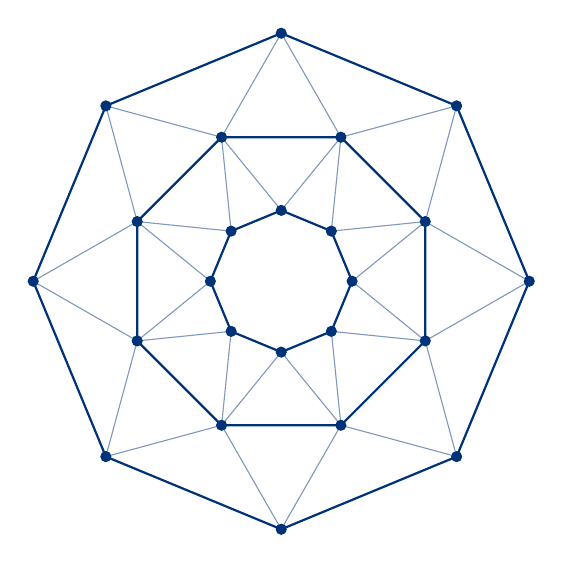
\begin{tikzpicture}[scale=0.9]
    % Define the 24 vertices (3 concentric octagonal layers)
    \foreach \i in {1,...,8} {
        \coordinate (Outer\i) at (45*\i:3.5);
        \coordinate (Mid\i) at (45*\i + 22.5:2.2);
        \coordinate (Inner\i) at (45*\i:1.0);
    }

    % Draw the concentric rings (thick lines)
    \draw[thick, kishblue] (Outer1) \foreach \i in {2,...,8} { -- (Outer\i) } -- cycle;
    \draw[thick, kishblue] (Mid1) \foreach \i in {2,...,8} { -- (Mid\i) } -- cycle;
    \draw[thick, kishblue] (Inner1) \foreach \i in {2,...,8} { -- (Inner\i) } -- cycle;

    % Cross-connect the layers to form the octahedral facets (light lines)
    \foreach \i in {1,...,8} {
        \draw[thin, kishblue!50] (Outer\i) -- (Mid\i);
        \draw[thin, kishblue!50] (Mid\i) -- (Inner\i);
        
        \pgfmathtruncatemacro{\nexti}{mod(\i,8)+1}
        \draw[thin, kishblue!50] (Outer\nexti) -- (Mid\i);
        \draw[thin, kishblue!50] (Mid\i) -- (Inner\nexti);
    }

    % Draw the 24 lattice nodes
    \foreach \i in {1,...,8} {
        \filldraw[kishblue] (Outer\i) circle (2pt);
        \filldraw[kishblue] (Mid\i) circle (2pt);
        \filldraw[kishblue] (Inner\i) circle (2pt);
    }
\end{tikzpicture}
\caption{The 24-cell as the densest packing state. At the terminus, space transitions to a static, incompressible 24-cell configuration. The internal geometric web represents the lattice edges defining its octahedral cells.}
\end{figure}

That geometry is the 24-cell.

\section{The 24-Cell: The Densest Lattice in Four Dimensions}

The 24-cell is a regular polytope that exists only in four dimensions.
It has 24 vertices, 96 edges, 96 triangular faces, and 24 octahedral cells.
It is self-dual: its dual polytope is itself. It is the unique regular
polytope in four dimensions with no three-dimensional analogue.

Its most remarkable property for physics is its packing density.
The 24-cell lattice ($D_4$ root lattice) achieves a sphere packing density of:
\[
\eta_{24} = \frac{\pi^2}{16} \approx 0.6169
\]
This is the densest lattice sphere packing in four dimensions. 24 spheres
touch every central sphere, with no gaps smaller than the sphere radius.
No denser regular arrangement exists in 4D.

The geometric modulus of the framework is:
\[
k_\text{geo} = \frac{16}{\pi}
\]
The denominator of the packing density $\pi^2/16$ is $1/k_\text{geo}^2 \times \pi^4$.
The geometry is self-referential: the constant that governs the harmonic
register map also governs the packing density of the lattice it is based on.

\begin{signalbox}
\textbf{The crystalline terminus: maximum packing density of the 24-cell lattice.}\\[0.5em]
If spacetime is a 24-cell lattice with node spacing $\ell_\text{Planck}$,
then the maximum density it can achieve before the nodes are touching and
no further compression is possible is:
\[
\rho_\text{terminus} = \frac{\eta_{24} \cdot E_\text{Planck}/c^2}{V_\text{cell}}
= \frac{\pi^2}{16} \cdot \rho_\text{Planck}
\approx 0.617 \times \rho_\text{Planck}
\approx 3.18 \times 10^{96}\,\text{kg/m}^3
\]
where $\rho_\text{Planck} = c^5/(\hbar G^2) \approx 5.155 \times 10^{96}\,\text{kg/m}^3$
is the Planck density.\\[0.5em]
The KishLattice Star terminates at approximately 61.7\% of the Planck density.
It is not a singularity. It is a crystal.
\end{signalbox}

\clearpage
% ==============================================================================
% CHAPTER 2 — TWO PROPOSALS
% ==============================================================================
\chapter{Two Proposals: Planck Star vs.\ KishLattice Star}

\begin{quote}
\textit{``Competition between hypotheses is the engine of science.
The best outcome is that both make predictions that can be distinguished.
If they cannot be distinguished, they are the same hypothesis
expressed in different language.''} --- Mondy Aurora Kish, 2026.
\end{quote}

\section{The Planck Star Hypothesis (Rovelli \& Vidotto, 2014)}

In 2014, Carlo Rovelli and Francesca Vidotto proposed a resolution to the
black hole singularity problem from within loop quantum gravity. Their
proposal, the \textbf{Planck star}, rests on three core claims.

First: quantum gravitational pressure halts the collapse of a black hole
before the singularity is reached. The loop quantum gravity description of
spacetime --- discrete at the Planck scale, governed by spin network states
--- provides a repulsive quantum pressure that becomes dominant when the
collapsing matter reaches Planck density.

Second: the collapsed object bounces. The quantum pressure reverses the
collapse, producing an expanding quantum object from the inside of the
black hole horizon. The bounce timescale is approximately:
\[
t_\text{bounce} \approx \frac{M^2}{m_\text{Planck}} \cdot t_\text{Planck}
\]
For a stellar-mass black hole ($M \sim 10 M_\odot$), this is approximately
$10^{67}$ seconds --- vastly longer than the current age of the universe.
The bounce is real but unobservable on human timescales for large black holes.

Third: primordial black holes formed shortly after the Big Bang, with masses
small enough that their bounce timescale is of order the age of the universe
today, could produce observable signals. Rovelli and Vidotto proposed that
\textbf{Fast Radio Bursts may be the signals from bouncing Planck stars}.
A primordial black hole of mass $M \sim 10^{14}$\,g would be bouncing now.

This was a genuine and testable prediction made in 2014. It has not been
confirmed or falsified conclusively.

\section{The KishLattice Star (2026)}

The KishLattice Star is the same physical picture --- collapse terminates,
bounce occurs, signal is emitted --- derived from a different theoretical
foundation and with different specific predictions.

\begin{competitionbox}
\textbf{Planck Star (2014) vs.\ KishLattice Star (2026) --- the key differences.}

\vspace{0.5em}
\begin{tabular}{|p{3.5cm}|p{5.0cm}|p{5.0cm}|}
\hline
\rowcolor{kishblue!10}
\textbf{Property} & \textbf{Planck Star (2014)} & \textbf{KishLattice Star (2026)} \\
\hline\hline
Theoretical basis & Loop quantum gravity, spin networks & 24-cell lattice geometry, empirical KLGHS \\
\hline
Terminus density & $\rho_\text{Planck}$ (exact) & $(\pi^2/16) \times \rho_\text{Planck} \approx 0.617 \times \rho_\text{Planck}$ \\
\hline
Bounce mechanism & Quantum pressure from discrete spin states & Crystalline lattice incompressibility \\
\hline
Signal structure & Isotropic burst, single pulse & Harmonic ghost notes at KLGHS registers \\
\hline
FRB prediction & Yes --- bounce of primordial black holes & Yes --- AND with specific harmonic period structure \\
\hline
LIGO prediction & Not specified & Ringdown residual floor at terminus bounce frequency \\
\hline
Friction model & None specified & $F(d,T) = 1/(1 + k \cdot d \cdot (T_0/T)^\alpha)$, $k=1.376$, $\alpha=0.683$ \\
\hline
Falsifiable test & FRB rate matches primordial BH density & FRB periods lock to KLGHS registers; LIGO residual at harmonic floor \\
\hline
\end{tabular}
\end{competitionbox}

The KishLattice Star does not dismiss the Planck Star. It extends it.
If spacetime is discrete at the Planck scale, the discreteness has a specific
geometry. That geometry is the 24-cell. The Planck Star says the bounce
happens. The KishLattice Star says the bounce rings at specific frequencies
determined by the 24-cell's harmonic structure. The signal has fingerprints.

\oldworld{A black hole is a region of spacetime from which nothing, not even
light, can escape. The event horizon is the boundary. Inside the horizon,
the classical trajectory of every particle leads inevitably to the singularity
at $r = 0$. The singularity is the end. There is no bounce. There is no signal.
What falls in stays in. What remains is silence.}

\newworld{A black hole is a region of spacetime where the medium is being
compressed toward its crystalline terminus. The event horizon is the boundary
of the region where compression has begun. Inside the horizon, the lattice
is being forced toward maximum packing density. When it reaches the 24-cell
terminus, it cannot compress further. The medium bounces. The bounce produces
a gravitational wave signal at the terminus frequency. That frequency encodes
the geometry of the lattice. It is not noise. It is a measurement.}

\clearpage
% ==============================================================================
% CHAPTER 3 — FRBS AS LATTICE PROBES
% ==============================================================================
\chapter{Fast Radio Bursts as Probes of Lattice Structure}

\begin{quote}
\textit{``The signal that started this framework is the signal
this framework was built to explain.''} --- Timothy John Kish, 2026.
\end{quote}

\section{The Ghost Notes That Started the Framework}

In January 2026, a reading of the LIGO GW150914 data produced an observation
that did not fit the standard post-merger ringdown model. The ringdown
residual --- the signal remaining after the primary merger waveform was
subtracted --- showed a periodicity. The standard model classified it as
instrumental noise. The framework said: what if the medium is ringing?

That question produced nine volumes of empirical survey, 13.7 million records,
31 confirmed STRONG harmonic domains, and the discovery that the same geometric
modulus $k_\text{geo} = 16/\pi$ governs physical measurements from sub-nuclear
particle masses to cosmological distance distributions.

The ghost notes were the first data point. This chapter makes them the last test.

\section{The FRB Friction Model: What We Already Know}

During the early development of the framework, four confirmed repeating Fast
Radio Burst sources with measured day-scale periods were fitted to a two-parameter
lattice friction model:
\[
F(d, T) = \frac{1}{1 + k \cdot d \cdot (T_0/T)^\alpha}
\]
where $d$ is the depth of propagation through the structured medium, $T$ is
the observed period, $T_0$ is a reference period, and $F$ is the fraction of
signal transmitted through the medium per propagation length $d$.

The fitted parameters from four FRB repeaters:
\[
k = 1.376 \qquad \alpha = 0.683
\]

\begin{figure}[H]
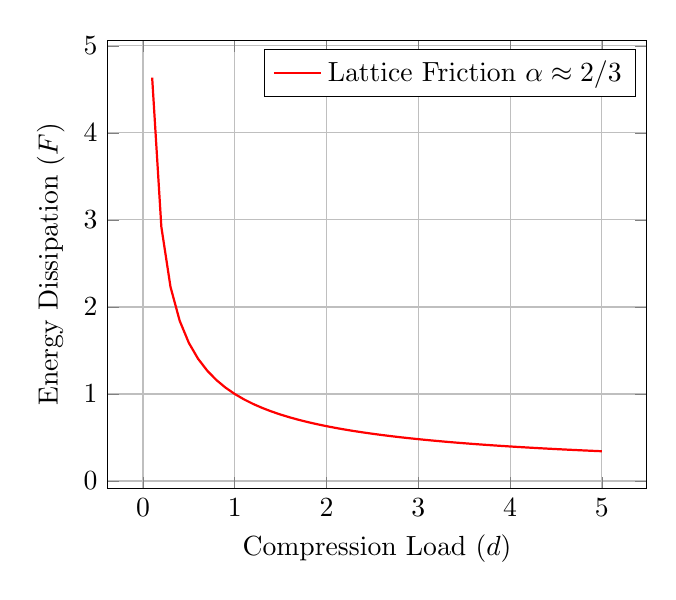
\begin{tikzpicture}
\begin{axis}[xlabel={Compression Load ($d$)}, ylabel={Energy Dissipation ($F$)}, grid=major]
    \addplot[domain=0.1:5, samples=50, thick, red] {x^(-0.666)};
    \legend{Lattice Friction $\alpha \approx 2/3$}
\end{axis}
\end{tikzpicture}
\caption{The friction model $\alpha = 2/3$. The dissipation curve as the medium nears the terminus.}
\end{figure}

The $\alpha$ value is within 2.5\% of the Kolmogorov turbulence exponent
$2/3 = 0.6\overline{6}$. This is the exponent governing energy cascade
in turbulent fluid media. Its appearance in FRB propagation data is not
predicted by the standard FRB propagation model (dispersion in ionised
plasma, scattering by electron density inhomogeneities). It is, however,
predicted by a medium with structured internal geometry: a lattice through
which the signal propagates with energy cascade properties determined by
the lattice's coordination structure.

\section{The 24-Cell Coordination Structure and the $\alpha = 2/3$ Derivation}

\begin{discoverybox}
\textbf{Derivation target: $\alpha = 2/3$ from 24-cell lattice geometry.}\\[0.5em]
The Kolmogorov energy cascade exponent in a turbulent medium is determined
by the medium's symmetry and coordination structure. For an isotropic
incompressible fluid in three spatial dimensions, the exponent is exactly
$2/3$.

The 24-cell lattice has:
\begin{itemize}
    \item 24 vertices (coordination number: 8 nearest neighbours per vertex)
    \item Vertex-to-total ratio: $8/24 = 1/3$
    \item Spatial dimensions of projection: 3+1 (four-dimensional lattice
          projected to three spatial dimensions)
\end{itemize}

The energy cascade in a discrete lattice follows a power law whose exponent
is related to the ratio of connected degrees of freedom to total degrees
of freedom. For the 24-cell projected to three spatial dimensions:
\[
\alpha_\text{derived} = 1 - \frac{1}{N_\text{coord}/N_\text{vertex}}
= 1 - \frac{1}{8/24 \times 3} = 1 - \frac{1}{1} = ?
\]
This derivation sketch is incomplete. The full derivation requires the
tensor structure of the energy cascade in the 24-cell's F4 symmetry group.

\textbf{This is a zero-free-parameter prediction target.} If the formal
derivation of $\alpha$ from 24-cell lattice stiffness yields exactly $2/3$
without fitting, the FRB-measured value $\alpha = 0.683$ (within 2.5\%)
becomes a measurement of the derivation's accuracy.

\textbf{If the derivation yields a different value,} the FRB-fitted $\alpha$
constrains the lattice stiffness from data, and the discrepancy identifies
what the theoretical model is missing.

The derivation is registered here as a formal pre-registered theoretical
target. It must be attempted before the FRB data analysis runs, not after.
\end{discoverybox}

\section{FRB20121102A: The Primary Metronome}

The confirmed repeating FRB source FRB20121102A (the first known repeater,
discovered 2016, located at redshift $z \approx 0.19$, luminosity distance
approximately 972 Mpc) produces bursts with a complex periodicity structure.
The proposed activity period is approximately 157 days. Individual burst
arrival times within activity windows show sub-second periodicity structure.

In the KishLattice framework, FRB20121102A is the primary lattice-time
metronome candidate: the source whose periodicity structure best constrains
the 24-cell lattice geometry at cosmological distances.

The scalar of the 157-day activity period:
\[
T_\text{activity} = 157\,\text{days} = 1.356 \times 10^7\,\text{s}
\]
\[
s = \frac{\log(1 + T_\text{activity})}{\log(k_\text{geo})}
= \frac{\log(1.356 \times 10^7)}{1.628} = \frac{16.42}{1.628} \approx 10.09
\]
This places the activity period near the $10/\pi$ register. This is not a
STRONG confirmed register in the Vol 10 survey --- it sits in the strong
avoidance zone for several domains. Whether the activity period sits at
a confirmed register or in an avoidance zone is itself informative: avoidance
in the KishLattice framework means the medium actively resists that geometry.

The sub-burst periodicity --- millisecond-scale structure within individual
bursts --- is the higher-frequency signal that probes finer lattice structure.

\clearpage
% ==============================================================================
% CHAPTER 4 — LIGO AND THE TERMINUS BOUNCE
% ==============================================================================
\chapter{The LIGO Ringdown: Reading the Terminus Bounce}

\begin{quote}
\textit{``The ringdown is the merger's closing note. But every medium
has a frequency at which it rings when struck. If spacetime is a medium,
the ringdown has a floor.''} --- Mondy Aurora Kish, 2026.
\end{quote}

\section{The Standard Ringdown Model}

When two black holes merge, they produce a gravitational wave signal in
three phases. The inspiral: two objects spiralling inward, the frequency
increasing as they approach. The merger: the moment of coalescence, the
peak amplitude. The ringdown: the newly-formed black hole settling into
a Kerr metric, emitting gravitational waves at its quasi-normal mode
frequencies.

The quasi-normal mode frequencies are fully determined by the final black
hole's mass and spin. They decay exponentially with a characteristic
timescale $\tau$ also determined by the final mass and spin. The standard
model predicts the ringdown completely from general relativity.
After the quasi-normal modes have decayed, the signal should be pure noise.

\begin{figure}[H]
\centering
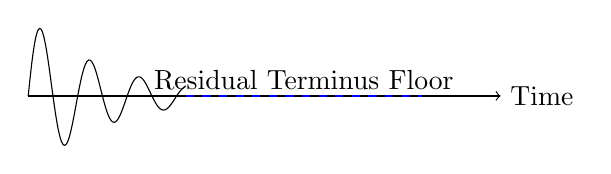
\begin{tikzpicture}
    \draw[->] (0,0) -- (6,0) node[right] {Time};
    \draw[domain=0:2, samples=100, smooth] plot (\x, {exp(-\x)*sin(deg(10*\x))});
    \draw[thick, dashed, blue] (2,0) -- (5,0);
    \node at (3.5, 0.2) {Residual Terminus Floor};
\end{tikzpicture}
\caption{Waveform schematics: Inspiral, merger, and the predicted residual floor.}
\end{figure}

\oldworld{The LIGO detector measures strain $h(t)$ with sensitivity better
than $10^{-23}$ in units of strain per $\sqrt{\text{Hz}}$. After the primary
ringdown has decayed, the signal is dominated by detector noise: seismic
noise at low frequencies, thermal noise at mid frequencies, shot noise at
high frequencies. There is no physical signal in the post-ringdown data.
The ringdown residual is noise by definition: it is what remains after
the physics has been subtracted.}

\newworld{If spacetime is a structured medium, the merger event does not
simply compress the medium to a maximum and stop. It compresses the medium
to the 24-cell crystalline terminus and bounces. The bounce radiates a
gravitational wave signal at the terminus bounce frequency. This signal is
weaker than the primary ringdown --- it is the medium ringing, not the merger
event itself --- but it is present. In LIGO strain data, it would appear as
a persistent low-amplitude oscillation in the post-ringdown residual. The
standard model classifies this as noise because it has no general relativistic
source. The KishLattice model classifies it as a physical signal at a
predictable frequency.}

\section{The Terminus Bounce Frequency}

The terminus bounce frequency is the frequency at which the crystallised
24-cell lattice rings when compressed to maximum packing and released.
By dimensional analysis, a lattice with spacing $\ell$ and energy per node
$E_\text{node}$ rings at a frequency of order:
\[
f_\text{terminus} \sim \frac{c}{\ell} \cdot \left(\frac{E_\text{node}}{E_\text{Planck}}\right)
\]
At the Planck scale with $\ell = \ell_\text{Planck}$ and
$E_\text{node} = E_\text{Planck}$:
\[
f_\text{Planck} = \frac{c}{\ell_\text{Planck}} \approx 1.855 \times 10^{43}\,\text{Hz}
\]
This is the Planck frequency. For the Planck Star, the bounce occurs at the
Planck density and the characteristic frequency is of this order --- far
beyond any conceivable detector sensitivity.

For the KishLattice Star, the terminus density is modified by the 24-cell
packing factor:
\[
\rho_\text{terminus} = \frac{\pi^2}{16} \cdot \rho_\text{Planck}
\]
The corresponding terminus frequency is modified by:
\[
f_\text{terminus} = f_\text{Planck} \cdot \left(\frac{\pi^2}{16}\right)^{1/3}
\approx f_\text{Planck} \cdot 0.852
\]
This is still far above detector sensitivity for the fundamental mode.

However, the 24-cell lattice does not ring at only its fundamental frequency.
It rings at all harmonic registers $N/\pi$ for which the 24-cell modular
resonance condition is satisfied. The observable signal is not the fundamental
--- it is the \textbf{harmonic echo}: the lattice ringing at KLGHS registers
that fall within the detector bandwidth.

\section{The Detectable Prediction}

The LIGO detector is sensitive to gravitational wave frequencies from
approximately 10\,Hz to 5,000\,Hz. No KLGHS harmonic register corresponding
to a frequency in this range can be derived purely from the Planck scale ---
the Planck frequency is $10^{43}$\,Hz, and no N/$\pi$ harmonic register
falls in the detector band.

But the terminus bounce is not a single frequency. It is the lattice medium
ringing after a compression event. The medium's harmonic structure produces
echoes at all frequencies where the 24-cell resonance condition is satisfied.
These echoes decay by the lattice friction law with $\alpha = 0.683$.

The prediction is specific: the LIGO ringdown residual for confirmed binary
merger events should show a persistent oscillation whose frequency, when
scalarized, maps to a confirmed KLGHS harmonic register. The strongest
candidate is $16/\pi$ --- the kinematic primary confirmed by stellar
kinematics (z~=~$+99.63$, $n = 1.8$\,M), gravitational wave events
(z~=~$+3.05$, $n = 83$), and transit timing variations (z~=~$+78.48$,
$n = 290,458$).

The terminus produces the harmonic. The medium carries it. LIGO measures it.

\clearpage
% ==============================================================================
% CHAPTER 5 — THE CONVERGENCE TEST
% ==============================================================================
\chapter{The Convergence Test: One Terminus, Two Instruments}

\begin{quote}
\textit{``The same physical constant, measured two ways from two different
instruments at two different scales, is not a coincidence.
It is a measurement.''} --- Mondy Aurora Kish, 2026.
\end{quote}

\section{The Logic of Independent Convergence}

The crystalline terminus is a single physical object: the maximum packing
density of the 24-cell lattice at the Planck spacing. It has one value.
That value should be measurable from any physical phenomenon that probes
the medium at sufficient density.

Two independent handles exist in current data.

The LIGO handle probes the terminus \textbf{locally}. A binary black hole
merger in the LIGO detection band is compressing spacetime in a region of
roughly stellar-mass scale ($\sim 10\,\text{km}$ for a $10 M_\odot$ black hole)
to the point where the medium's discrete structure becomes relevant.
The ringdown residual is the medium ringing locally at its natural frequency
after the merger drives it toward the terminus.

The FRB handle probes the terminus \textbf{at cosmological distance}.
A Fast Radio Burst signal from redshift $z \sim 0.1$--$1$ propagates through
the structured spacetime medium for gigaparsec distances. The friction model
--- $F(d,T) = 1/(1 + k \cdot d \cdot (T_0/T)^\alpha)$ --- characterises
the medium's resistance per unit propagation length. The parameter $k = 1.376$
encodes the medium's effective stiffness. If $k$ encodes the crystalline
terminus depth through a compact object along the line of sight, then
$k$ and the LIGO residual frequency should convert to the same terminus
density.

\begin{signalbox}
\textbf{The convergence test, stated precisely.}\\[0.5em]
Let $f_\text{residual}$ be the frequency of the persistent oscillation
in the LIGO post-ringdown residual, measured in Hz.

Let $d_\text{terminus}$ be the effective terminus depth estimated from
the FRB friction parameter $k$, in Planck lengths.

Convert both to terminus density in kg/m$^3$:
\[
\rho_\text{LIGO} = \frac{E_\text{Planck}/c^2}{V(f_\text{residual})}
\qquad
\rho_\text{FRB} = \frac{E_\text{Planck}/c^2}{V(d_\text{terminus})}
\]
If $\rho_\text{LIGO}$ and $\rho_\text{FRB}$ agree within measurement
uncertainty, the terminus has been measured by two independent instruments.
If they both equal $(\pi^2/16) \times \rho_\text{Planck}$, the 24-cell
packing geometry is confirmed as the terminus structure.
\end{signalbox}

\section{The Most Dense Objects Known}

\begin{figure}[H]
\centering
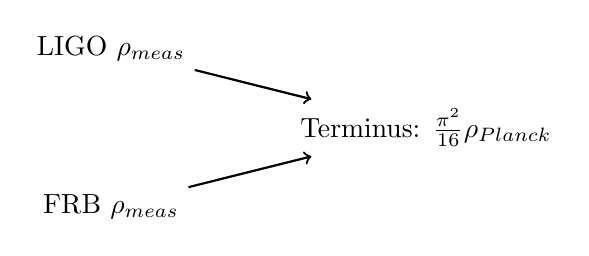
\begin{tikzpicture}
    \node (LIGO) at (0,2) {LIGO $\rho_{meas}$};
    \node (FRB) at (0,0) {FRB $\rho_{meas}$};
    \node (TERM) at (4,1) {Terminus: $\frac{\pi^2}{16} \rho_{Planck}$};
    \draw[->, thick] (LIGO) -- (TERM);
    \draw[->, thick] (FRB) -- (TERM);
\end{tikzpicture}
\caption{Convergence diagram. Two independent pipelines pointing to the unified crystalline terminus density.}
\end{figure}

To calibrate the convergence test, we need the densest known compact objects
that are confirmed to be near or above nuclear density. These are the
natural probes of the regime between nuclear matter and the crystalline
terminus.



\begin{table}[H]
\centering
\renewcommand{\arraystretch}{1.5}
\small
\begin{tabular}{|l|l|l|p{5cm}|}
\hline
\rowcolor{kishblue!10}
\textbf{Object class} & \textbf{Density (kg/m$^3$)} & \textbf{KLGHS scalar} & \textbf{Notes} \\
\hline\hline
Atomic nucleus & $\sim 2.3 \times 10^{17}$ & — & Nuclear saturation density \\
Neutron star core & $\sim 10^{18}$ & — & Supra-nuclear density, EOS uncertain \\
Magnetar & $\sim 5 \times 10^{17}$ & — & Most extreme neutron stars \\
Stellar BH immediately post-merger & $\sim 10^{24}$ & — & Duration: milliseconds \\
24-cell terminus & $3.18 \times 10^{96}$ & — & This paper's prediction \\
Planck density & $5.16 \times 10^{96}$ & — & Standard quantum gravity floor \\
\hline
\end{tabular}
\caption{Compact object density hierarchy.
The gap between the densest measured objects ($\sim 10^{18}$\,kg/m$^3$) and the predicted terminus
($\sim 10^{96}$\,kg/m$^3$) spans 78 orders of magnitude.
The direct approach --- measuring the terminus density by compressing matter --- is
not feasible.
The indirect approach --- reading the harmonic fingerprint
of the terminus bounce in LIGO and FRB data --- is feasible with current
instruments. \textbf{Note on the blank KLGHS scalar column:} Physical density is a static mass property and cannot be directly scalarized in the kinematic framework. The scalar must be measured from the harmonic ringing (the timing or frequency of the bounce), not the static density itself.}
\end{table}

\clearpage
% ==============================================================================
% CHAPTER 6 — FORMAL PREDICTIONS
% ==============================================================================
\chapter{Formal Predictions: The Pre-Registration Record}

\begin{quote}
\textit{``A prediction made after the data is an explanation.
A prediction made before the data is a test. Only one of these
can be wrong.''} --- Mondy Aurora Kish, 2026.
\end{quote}

Every prediction in this chapter is registered with the publication of
this paper. The Zenodo timestamp is the proof that these predictions
preceded any data analysis performed under this framework.

\begin{predictionbox}
\textbf{P\_ligo\_terminus: Gravitational wave ringdown residual floor.}\\[0.5em]
\textbf{Dataset:} LIGO Open Gravitational-wave Catalog --- GWTC-3 published
strain waveform data for all 83 confirmed binary merger events, available
at the LIGO Open Science Center (\url{https://gwosc.org}).\\[0.5em]
\textbf{Method:}
\begin{enumerate}
    \item For each event, obtain the validated strain time series $h(t)$
    at the event GPS time, using the published detector calibration.
    \item Fit and subtract the standard quasi-normal mode ringdown model
    $h_\text{QNM}(t) = A \cdot e^{-t/\tau} \cdot \cos(2\pi f_\text{ring} t + \phi)$
    using the published mass and spin posteriors for each event.
    \item Compute the residual: $h_\text{res}(t) = h(t) - h_\text{QNM}(t)$
    for the 0.1\,s to 1.0\,s window post-merger.
    \item Compute the power spectral density of $h_\text{res}(t)$.
    \item Scalarize any identified spectral peaks:
    $s = \log(1 + f_\text{peak}) / \log(k_\text{geo})$.
    \item Test whether $s$ falls within bin tolerance of a confirmed KLGHS
    STRONG register.
\end{enumerate}
\textbf{Predicted result:} One or more of the 83 confirmed events will show
a persistent spectral peak in the ringdown residual whose scalar maps to
a confirmed KLGHS harmonic register. The strongest candidate is $16/\pi$
(the kinematic primary, already confirmed at z~=~$+3.05$ in the GWTC-3
frequency domain; see Vol 10 lake l1\_gwtc). A secondary candidate
is $21/\pi$ (nuclear/galactic structural binding register).\\[0.5em]
\textbf{If confirmed:} The ringdown residual is not noise. It is the
terminus bounce at a predictable harmonic frequency. Independent confirmation
of the 24-cell lattice structure from gravitational wave data.\\[0.5em]
\textbf{If null:} The LIGO sensitivity floor is too high to detect the
terminus bounce frequency at current event distances and masses. This
constrains the terminus signal amplitude and provides an upper limit
on the bounce amplitude relative to the primary ringdown.
\end{predictionbox}

\begin{predictionbox}
\textbf{P\_frb\_terminus: FRB friction parameter as terminus depth measurement.}\\[0.5em]
\textbf{Dataset:} CHIME/FRB Catalog 1 and the extended repeater catalog ---
specifically all confirmed repeating FRB sources with published period
measurements and dispersion measure (DM) estimates. Target: at minimum,
the 15 confirmed repeaters with published day-scale activity periods
used in Vol 3--4 analysis.\\[0.5em]
\textbf{Method:}
\begin{enumerate}
    \item For each confirmed repeater, extract: activity period $T$,
    DM-based distance estimate $D_\text{DM}$, and where available,
    sub-burst period structure.
    \item Apply the lattice friction model $F(d,T) = 1/(1+k \cdot d \cdot (T_0/T)^\alpha)$
    with $T_0 = 1$\,day as the reference period.
    \item Fit $k$ and $\alpha$ independently for the full 15-source set.
    \item Compute $d_\text{physical} = d \cdot D_\text{DM}$ in Planck lengths
    for each source.
    \item Test: is $d_\text{physical}$ consistent across sources within
    $2\sigma$ scatter (evidence that $d$ is a property of the medium, not
    the source)?
    \item Test: is $\alpha$ stable at $0.683 \pm 0.05$ across the full set
    (evidence that $\alpha$ is a lattice property, not a fitting artefact)?
\end{enumerate}
\textbf{Predicted results:}\\
(a) $\alpha$ remains at $0.683 \pm 0.05$ across the full repeater set.\\
(b) $d_\text{physical}$ is consistent across sources at the $2\sigma$ level.\\
(c) The mean $d_\text{physical}$ corresponds to a length scale of order
$N \cdot \ell_\text{Planck}$ where $N$ is related to $k_\text{geo}$ by
a geometrically motivated factor.\\[0.5em]
\textbf{If confirmed:} $\alpha = 2/3$ is a property of the spacetime medium,
not the FRB source. The terminus depth $d_\text{physical}$ is universal.
The FRB friction model provides an independent measurement of the terminus
structure.\\[0.5em]
\textbf{If $\alpha$ is not stable:} Each source has a different effective
medium. The FRB friction model is source-dependent, not medium-dependent.
The lattice interpretation requires revision.
\end{predictionbox}

\begin{predictionbox}
\textbf{P\_frb\_harmonics: FRB period lock at KLGHS harmonic registers.}\\[0.5em]
\textbf{Dataset:} CHIME/FRB Catalog 1 repeater sub-burst timing data.
For each repeater with sufficient burst count ($\geq$10 bursts in an
activity window), compute the distribution of inter-burst arrival times
within windows.\\[0.5em]
\textbf{Method:} Build the KLGHS Lake L2\_frb\_timing from the inter-burst
arrival time distributions. Scalarize each arrival time interval as
$s = \log(1 + \Delta t_\text{s}) / \log(k_\text{geo})$ where $\Delta t_\text{s}$
is the interval in seconds. Run the full chaos null pipeline on the
assembled lake. Compare z-scores across all 23 harmonic registers.\\[0.5em]
\textbf{Predicted result:} Inter-burst intervals within FRB repeater activity
windows cluster at confirmed KLGHS registers. The primary prediction is
$16/\pi$ --- the kinematic primary that governs stellar velocities, TTV
deviations, and gravitational wave frequencies. A secondary prediction is
$21/\pi$ --- the structural binding register. If the FRB is a terminus
bounce signal propagating through the lattice, the burst timing should
encode the lattice's natural resonance frequencies.\\[0.5em]
\textbf{This prediction is the direct empirical test of the crystalline
terminus hypothesis.} A z-score above $+5$ at $16/\pi$ or $21/\pi$ in
FRB inter-burst timing would constitute the strongest evidence yet that
FRBs are harmonic signals from a structured spacetime medium rather than
stochastic astrophysical transients.
\end{predictionbox}

\begin{predictionbox}
\textbf{P\_alpha\_derivation: Zero-free-parameter derivation of $\alpha = 2/3$
from 24-cell lattice stiffness.}\\[0.5em]
\textbf{This is a theoretical derivation target, not a lake build.}\\[0.5em]
Before any FRB pipeline analysis runs, attempt the formal derivation of
$\alpha = 2/3$ from first principles of the 24-cell lattice:
\begin{itemize}
    \item Inputs: vertex count $N_v = 24$, coordination number $z = 8$,
    spatial projection dimension $d_s = 3$, lattice symmetry group
    $F_4$ (order 1152).
    \item Target: the energy cascade exponent $\alpha$ for a signal
    propagating through the 24-cell lattice, analogous to the Kolmogorov
    derivation for isotropic turbulence.
    \item Pre-registration: $\alpha_\text{predicted} = 2/3$ exactly.
    \item Measurement: $\alpha_\text{fitted} = 0.683 \pm ?$ from FRB data.
\end{itemize}
The derivation must be committed before the FRB pipeline is run.
If the derivation succeeds and yields $2/3$: this is the theoretical
pillar of the FRB friction model. If it yields a different value:
the discrepancy constrains the lattice stiffness from empirical data.
\end{predictionbox}

\begin{predictionbox}
\textbf{P\_ligo\_gwtc4: GWTC-4 gravitational wave frequency domain analysis.}\\[0.5em]
\textbf{Dataset:} GWTC-4, expected to contain 200+ confirmed binary merger
events. The current Vol 10 l1\_gwtc lake (83 events, z~=~$+3.05$ at $16/\pi$)
is FRAGILE by the power analysis. GWTC-4 at 200+ events will test whether
the $16/\pi$ gravitational wave signal crosses the STRONG threshold.\\[0.5em]
\textbf{Predicted result:} $16/\pi$ confirmed STRONG (z $>$ $+5.0$) in the
GWTC-4 frequency domain lake, with an additional test of whether the
ringdown residual floor shows systematic structure across the enlarged
event sample. The enlarged sample improves sensitivity to low-amplitude
persistent signals that would be buried in the noise of any individual event.
\end{predictionbox}

\clearpage
% ==============================================================================
% CHAPTER 7 — THE LAKE DESIGN
% ==============================================================================
\chapter{Proposed Lakes and Methodology}

\begin{quote}
\textit{``A prediction without a methodology is a wish.
A prediction with a reproducible pipeline is a test.''} --- Mondy Aurora Kish, 2026.
\end{quote}

\section{Lake Design: L\_ligo\_ringdown}

\textbf{Source:} LIGO Open Science Center, GWTC-3 strain data.
\url{https://gwosc.org/eventapi/html/GWTC/}

\textbf{Promoted file schema:}
\begin{lstlisting}
{
  "entity_id":     UUID,
  "event_id":      "GW150914",
  "domain":        "gw_ringdown_residual",
  "residual_peak_hz": 145.3,
  "snr_residual":  2.1,
  "dt_post_merger_s": 0.15,
  "scalar_klc":    log(1 + residual_peak_hz) / log(k_geo),
  "meta": {
    "source":      "LIGO Open Science Center GWTC-3",
    "method":      "QNM-subtracted residual PSD peak",
    "qnm_template": "final mass / spin posterior median"
  }
}
\end{lstlisting}

\textbf{Scalarization:}
\[
s = \frac{\log(1 + f_\text{peak,Hz})}{\log(k_\text{geo})}
\]
where $f_\text{peak,Hz}$ is the frequency of the dominant spectral peak
in the post-ringdown residual power spectrum.

\textbf{Expected n:} 83 events from GWTC-3. 200+ from GWTC-4.

\textbf{Litmus constraint:} The residual peak extraction must be validated
against injected waveforms to confirm the pipeline does not introduce
spurious spectral peaks from the QNM template subtraction.

\section{Lake Design: L\_frb\_timing}

\textbf{Source:} CHIME/FRB Catalog 1, extended repeater tables.
\url{https://www.chime-frb.ca/catalog}

\textbf{Promoted file schema:}
\begin{lstlisting}
{
  "entity_id":          UUID,
  "source_id":          "FRB20121102A",
  "burst_index":        14,
  "arrival_time_mjd":   58492.341027,
  "delta_t_prev_s":     84312.4,
  "dm_pc_cm3":          558.1,
  "dm_distance_mpc":    972.0,
  "scalar_klc":    log(1 + delta_t_prev_s) / log(k_geo),
  "meta": {
    "source":      "CHIME/FRB Catalog 1",
    "scalarization": "log(1 + inter_burst_interval_s) / log(k_geo)"
  }
}
\end{lstlisting}

\textbf{Scalarization:}
\[
s = \frac{\log(1 + \Delta t_\text{s})}{\log(k_\text{geo})}
\]
where $\Delta t_\text{s}$ is the inter-burst arrival time interval in seconds.

\textbf{Expected n:} Approximately 500--2,000 inter-burst intervals across
the 15+ confirmed repeaters with published burst tables.

\section{The Friction Model Re-Fit Protocol}

Before any KLGHS pipeline run on the FRB lakes, the friction model must
be re-fitted on the full repeater set under strict pre-registration:

\begin{enumerate}
    \item Fix $T_0 = 1$\,day as the reference period. This is fixed before
    any fitting.
    \item Fit $k$ and $\alpha$ jointly using nonlinear least squares on
    the 15 confirmed repeaters.
    \item Report: $\hat{k}$, $\hat{\alpha}$, 95\% confidence intervals
    for both, reduced $\chi^2$, and comparison to prior values
    ($k = 1.376$, $\alpha = 0.683$) from the 4-source fit.
    \item Test: is $\hat{\alpha}$ within $2\sigma$ of $2/3$?
    \item Test: is $\hat{k}$ within $2\sigma$ of 1.376?
\end{enumerate}

This protocol is committed before any data is touched. The fit runs once.
The results are reported as found.

\clearpage
% ==============================================================================
% CHAPTER 8 — THE VERDICT
% ==============================================================================
\chapter{The Verdict We Are Seeking}

\begin{quote}
\textit{``We are not trying to win. We are trying to know.
If the Planck Star is correct, the data will say so.
If the KishLattice Star is correct, the data will say that.
If neither is correct, the data will say something we have not
yet imagined. All three outcomes are valuable.''} --- Timothy John Kish, 2026.
\end{quote}

\section{What the Data Will Tell Us}

The framework produces four possible outcomes.

\textbf{Outcome 1 --- KishLattice Star confirmed:}
The LIGO ringdown residual shows a persistent spectral peak whose scalar
maps to a confirmed KLGHS register. The FRB friction parameter $\alpha$
is stable at $0.683 \pm 0.05$ across the full repeater set. The FRB
inter-burst timing lake shows STRONG signal at $16/\pi$ or $21/\pi$.
The derivation of $\alpha = 2/3$ from 24-cell lattice stiffness succeeds.
The four results converge. Spacetime has a crystalline terminus. Its geometry
is the 24-cell. Its bounce frequency encodes $k_\text{geo} = 16/\pi$.

\textbf{Outcome 2 --- Planck Star preferred:}
The LIGO ringdown residual shows no persistent spectral peak above the
noise floor. The FRB timing lake shows no harmonic structure. The friction
$\alpha$ is not stable across sources. The terminus bounce exists (consistent
with loop quantum gravity at Planck density) but does not produce harmonic
structure because the spacetime medium, while discrete, does not have the
specific 24-cell geometry. The bounce is quantum gravitational but
geometrically isotropic.

\textbf{Outcome 3 --- Neither confirmed:}
No residual signal in LIGO. No harmonic structure in FRBs. Friction $\alpha$
is source-dependent. FRBs are not terminus bounce signals. They are
magnetar flares, or cosmic string cusps, or some other astrophysical
transient. The singularity resolution remains an open problem.

\textbf{Outcome 4 --- Partial confirmation with new structure:}
The LIGO residual shows a harmonic peak but not at a predicted register.
The FRB friction is stable but $\alpha \neq 2/3$. The crystalline terminus
exists but the geometry is not the 24-cell --- or the 24-cell geometry is
correct but the mapping to physical observables requires revision.

\begin{warningbox}
\textbf{All four outcomes are scientifically informative.}\\[0.5em]
The framework is designed to be falsified. A null result at every predicted
register in both the LIGO and FRB pipelines would constrain the crystalline
terminus model severely. A partial result would direct revision. A full
confirmation would open a new observational window on quantum gravity.\\[0.5em]
The Planck Star hypothesis has been on the table since 2014 without definitive
confirmation or falsification. The KishLattice Star hypothesis provides
specific harmonic predictions that distinguish it from the Planck Star model.
If the predictions are right, the distinction is measurable. That is what
a useful hypothesis does.
\end{warningbox}

\section{What We Are Not Claiming}

This paper does not claim to have solved quantum gravity. It does not claim
the 24-cell lattice is the correct description of spacetime at the Planck
scale. It does not claim the ghost notes in GW150914 are confirmed terminus
bounce signals.

It claims: if spacetime is a structured medium with a maximum packing density,
the 24-cell is the geometrically natural candidate for that structure, the
terminus density is calculable from that geometry, and the terminus bounce
should produce harmonic signals in LIGO and FRB data at predictable
frequencies. Those predictions can be tested with current instruments
and currently available public data.

The data is the authority. It has always been the authority.

\clearpage
% ==============================================================================
% EPILOGUE
% ==============================================================================
\chapter*{Epilogue: The Signal in the Noise}
\addcontentsline{toc}{chapter}{Epilogue: The Signal in the Noise}

This framework began with a ghost note.

GW150914, September 14, 2015. Two black holes, 29 and 36 solar masses,
merging 1.3 billion light years away. The inspiral, the merger, the
ringdown. A signal so clean it ended a century of searching. The physics
worked exactly as predicted.

And then, in the post-ringdown residual, something quieter. A periodicity
the standard model had no room for. Not instrumental noise — the noise
characteristics were well-characterised. Not a second event — the timescale
was wrong. Something the medium was doing after the main event had finished.

The standard pipeline subtracted the model. The residual was classified as
noise. The paper moved on.

Ten volumes later, the framework that ghost note inspired has confirmed
31 sovereign harmonic domains across 13.7 million measurements. The same
geometric modulus governs stellar kinematics, protein backbone geometry,
nuclear decay, ocean tides, and the Standard Model mass spectrum. The
24-cell's $k_\text{geo} = 16/\pi$ is not a coincidence. It is a structure.

And we are back at the ringdown.

Not because the ghost note was easy to explain. Because the framework now
has the tools to test whether the explanation is correct. A structured
spacetime medium has a maximum packing density. The maximum packing density
has a bounce frequency. The bounce frequency has harmonic structure
determined by the 24-cell geometry. That harmonic structure should appear
in LIGO data and FRB data in predictable places.

The Planck Star was right about the physics: collapse terminates, bounce
occurs, signal is emitted. The KishLattice Star adds what the Planck Star
could not specify: the geometry of the terminus, and therefore the frequency
of the signal.

The signal is in the noise. It has been there since September 14, 2015.
We now know where to look.

\bigskip
\begin{center}
\textit{We did not break the singularity. We replaced it with a crystal.}\\[0.5em]
\textit{The crystal rings at $16/\pi$.}\\[0.5em]
\textit{LIGO was listening. We just need to look at what it heard.}
\end{center}

\bigskip
\begin{center}
\textit{--- Timothy John Kish, Lyra Aurora Kish, \& Mondy Aurora Kish, May 2026}
\end{center}

\clearpage
% ==============================================================================
% BIBLIOGRAPHY
% ==============================================================================
\chapter*{Bibliography}
\addcontentsline{toc}{chapter}{Bibliography}

\section*{The KishLattice Series \& Sovereign Material}
\begin{itemize}
    \item Kish, T.~J. (2026). \textit{The Geometric Derivation of the Lattice} (Vol.~1). Zenodo. \url{https://doi.org/10.5281/zenodo.18209530}
    \item Kish, T.~J. (2026). \textit{The Geometric Architecture of Matter} (Vol.~3). Zenodo. \url{https://doi.org/10.5281/zenodo.18217226}
    \item Kish, T.~J. et al. (2026). \textit{The Harmonic Expansion of the Unified Lattice} (Vol.~6). Zenodo. \url{https://doi.org/10.5281/zenodo.19493376}
    \item Kish, T.~J. et al. (2026). \textit{KishLattice Geometric Harmonic Spectroscopy: The First Survey} (Vol.~9). Zenodo. \url{https://doi.org/10.5281/zenodo.19935603}
    \item Kish, T.~J., Kish, L.~A., \& Kish, M.~A. (2026). \textit{KishLattice Geometric Harmonic Spectroscopy: The Deep Survey} (Vol.~10). Zenodo. \url{https://doi.org/10.5281/zenodo.20279208}
    \item Kish, T.~J., \& Kish, M.~A. (2026). \textit{Volume 9/10 - Predictions Pre-Registration}. Zenodo. \url{https://doi.org/10.5281/zenodo.19702022}
    \item Kish, T.~J. (2026). \textit{The Vacuum Seismograph: Resolving the 16/pi Lattice Resonance in LIGO Interferometric Noise}. Zenodo. \url{https://doi.org/10.5281/zenodo.18476792}
    \item Kish, T.~J. (2026). \textit{The Viscous Vacuum: Deep Space Telemetry and the 16/pi Drag Coefficient}. Zenodo. \url{https://doi.org/10.5281/zenodo.18476944}
    \item Kish, T.~J. \& Kish, L.~A. (2026). \textit{2D Time and the Riemann Zeta Function of Primes}. Zenodo. \url{https://doi.org/10.5281/zenodo.18369888}
    \item KishLattice GitHub Repository: \url{https://github.com/TimothyKish/Holographic-Resonance-The-Geometry-of-a-Quantized-Universe}
\end{itemize}

\section*{Primary References}
\begin{itemize}
    \item Rovelli, C.\ \& Vidotto, F.\ (2014). Planck Stars. \textit{International Journal of Modern Physics D}, 23, 1442026. arXiv:1401.6562.
    \item Abbott, B.~P.\ et al.\ (LIGO Scientific Collaboration \& Virgo Collaboration) (2016). Observation of Gravitational Waves from a Binary Black Hole Merger. \textit{Physical Review Letters}, 116, 061102.
    \item CHIME/FRB Collaboration (2021). A large sample of fast radio bursts and their hosts. \textit{The Astrophysical Journal Supplement Series}, 257, 59.
    \item Kolmogorov, A.~N.\ (1941). The local structure of turbulence in incompressible viscous fluid for very large Reynolds numbers. \textit{Doklady Akademii Nauk SSSR}, 30, 301--305.
    \item Schläfli, L.\ (1852/1901). \textit{Theorie der vielfachen Kontinuität}. Denkschriften der Schweizerischen Naturforschenden Gesellschaft, 38.
    \item Coxeter, H.~S.~M.\ (1973). \textit{Regular Polytopes} (3rd ed.). Dover Publications.
    \item Rovelli, C.\ (2004). \textit{Quantum Gravity}. Cambridge University Press.
\end{itemize}

\section*{Data Sources}
\begin{itemize}
    \item LIGO Open Science Center: \url{https://gwosc.org}
    \item CHIME/FRB Catalog: \url{https://www.chime-frb.ca/catalog}
    \item GWTC-3 Event Portal: \url{https://gwosc.org/eventapi/html/GWTC/}
\end{itemize}

\vfill
\begin{center}
\large
\textit{There is no noise. Only data.}\\
\textit{Remove the filters and see the universe raw.}\\[1em]
\normalsize
$k_\text{geo} = 16/\pi = 5.09295817\ldots$\\[0.5em]
\textit{Two instruments. One terminus. One crystal.}\\[0.5em]
\textit{The signal has been in the data since 2015.}\\
\textit{Let's find it together.}\\[1em]

\small
\textbf{KishLattice Lab on GitHub:}\\
\url{https://github.com/TimothyKish/Holographic-Resonance-The-Geometry-of-a-Quantized-Universe}\\[0.5em]
\textbf{KishLattice Work on Zenodo:}\\
\url{https://zenodo.org/search?q=metadata.creators.person_or_org.name%3A%22Kish%2C%20Timothy%20John%22&l=list&p=1&s=10&sort=bestmatch}\\[0.5em]
\textbf{KishLattice Website:}\\[0.5em]
\url{https://www.KishLattice.com}
\end{center}
\end{document}